%%%%%%%%%%%%%%%%%%%%%%%%%%%%%%%%%%%%%%%%%%%%%%%%%%%%%%%%%%%%
%%%%%%%%%%%%%%%%%%%%%%%%%%%%%%%%%%%%%%%%%%%%%%%%%%%%%%%%%%%%
\chapter{Application of  the WSME model to Myotrophin}
\label{chap:wsme-results}
\nopagebreak
%%%%%%%%%%%%%%%%%%%%%%%%%%%%%%%%%%%%%%%%%%%%%%%%%%%%%%%%%%%%
%%%%%%%%%%%%%%%%%%%%%%%%%%%%%%%%%%%%%%%%%%%%%%%%%%%%%%%%%%%%

In this chapter we report results of the application of the WSME model, described
%previously 
in chapter \ref{chap:wsme-model}, to the \emph{in silico} characterization of
the equilibrium and the kinetics of Myotrophin (pdb code: 2myo), an ankyrin
repeat protein  exhibiting a three-dimensional structure composed by the
repetition of a simple motif, while this modular characteristic is not clearly
reflected in the protein sequence.


%%+++++++++++++++++++++++++++++++++++++++++++++++++++++++++++++++
\section{Equilibrium}
%\subsection{Myotrophin presents a multi-minima free-energy profile, yet an apparent two-state behaviour.}


The order parameter $p(z)$ which is defined in Equation \ref{eq:ordpar_p}, as a
function of the denaturant factors $z$, temperature
or urea concentration, presents a classical sigmoidal shape, see Figure
\ref{fig:den-fit}.
Such curve provide a global information on the protein at the equilibrium and
this can be
interpreted as a two-state-like protein behaviour.
The resulting order parameter shape if found to be even sharper than the
experimental data maybe due to the model energy function that tends to enhance
cooperativity \cite{Abe2006}.

Experimentally, folding cooperativity is inferred when the molecule present
similar temperature behaviour of different observables, possibly giving local
and global information on the protein structure.
%both globally an locally the same order parameter behaviour.
To mimic the experimental procedure, in Figure \ref{fig:SI_p+W8}, we compare the
global order parameter signal $p(c)$, which can be associated to the far-UV CD band
used in Ref.~\cite{Mosavi2002a,Lowe2007a}, to the order parameter restricted to
the Tryptophan on the site 8 ($p_8(c)$), which can be related to the fluorescent
signal of Trp8.
The latter can be calculated analogously  to the global order parameter, substituting the
global $m$ with $\langle m_8\rangle$ and using its baselines.
The two curves overlap to a great extent which experimentally is usually
interpreted as two-state behaviour. 
\begin{figure}
\centering
%\includegraphics[width=3cm,angle=-90]{./img/wsme/res_denat-trp8}
\resizebox{0.6\textwidth}{!}{\sffamily\input{./img/wsme/graph-denat-trp8}}
\caption{Comparison of the signals of the order parameter $p$,
Equation~\ref{eq:ordpar_p}, and $p_8$ as functions of the denaturant concentration. 
These signals are somewhat analogous to the experimental measures of far-UV CD
band and of the fluorescent signal from Trp8.
Notice that the two signals present great agreement which is usually interpreted
in support of two-state behaviour, even if
some differences are evident below $c_m$.}
\label{fig:SI_p+W8}
\end{figure}


%%+++++++++++++++++++++++++++++++++++++++++++++++++++++++++++++++
\subsection{Multi-minima Free-energy Profile}
\label{subsec:prof}

On the other hand, while analysing the free-energy profiles, as a function of the fraction of native
residues $\rho=\frac MN$ one observe four minima, in both strongly renaturing and denaturating
conditions as shown in Figure~\ref{fig:eq}.
\begin{figure}
\centering
\subfigure[]{
\includegraphics[angle=-90,width=0.4\textwidth]{./img/wsme/prof-fold.eps}}
\subfigure[]{             
\includegraphics[angle=-90,width=0.4\textwidth]{./img/wsme/prof-unfold.eps}}
\caption{Examples of the Myotrophin free-energy profiles as a function of
the fraction of native residues $ \rho = M/N$. Panel \emph{a}: renaturing conditions
($c$=0). Panel \emph{b}: denaturing conditions ($c$=12). Despite the global
cooperativity of the folding process found in the order parameter analysis, the
free-energy profile present a multi-minima behaviour, suggesting the present of
low populated intermediate states. With the wild type curve (black) the behaviour
of destabilizing mutation are reported. Mutation destabilize respectively
N-terminal region (red line), central region (green line) and C-terminal region
(blue line).}
\label{fig:eq}
\end{figure}

The protein two-state-like behaviour that implies cooperative folding seem to be
in contradiction with the resulting multi-minima energy profile, for which one
can expect the presence of intermediates.
In the wild type species, where this behaviour is found, this apparent puzzle is
solved by observing that for most temperatures or denaturant concentrations, the
intermediate minima are found at a free-energy higher than the native or
unfolded minima, and almost
never become sufficiently populated to affect the two-state effective behaviour
of $p(z)$.

\begin{figure}
\centering
\subfigure[Total]{
\label{fig:SI_p_fits}
\includegraphics[angle=-90,width=0.4\textwidth]{./img/wsme/res_fit-2stati-tot-6par.eps}}
\subfigure[Trp8]{
\label{fig:SI_W8_fits}
%\psfrag{m8}{$\langle m_8\rangle$}
\includegraphics[angle=-90,width=0.4\textwidth]{./img/wsme/res_fit-2stati-trp-6par.eps}}
\caption{Fits of the fraction of native residues $m$ with a three-state model
(blue line),  with a two-state model and two parameters (green), and with a
two-state model and 6 parameters (purple) in the case of chemical denaturation. 
%In the two-parameters, two-state model the $m(c)$ signal is written as
%$m(c)=m_N f_N+ m_U f_U$, with the native state probability $f_N = (1+\exp(-\beta
%\Delta G_{U-N}))^{-1}$ and $f_U=1-f_N$. The free-energy difference between the U
%and N state is represented as $ \Delta G_{U-N}=\Delta G^0 + \gamma c$, with $
%\Delta G^0$ and $\gamma$ the fitting parameters.  The baselines $m_N$, $m_U$ are
%linear in $c$, and are previously estimated from separate fits of the $m(c)$
%signal at low and high concentration regions, far from the transition. In the
%three-state model, $m(c)=m_N f_N+ m_I f_I+ m_U f_u$,  $f_N =1/Z$,
%$f_I=\exp(-\beta \Delta G_{I-N})/Z$, $f_U=\exp(-\beta \Delta G_{U-N})/Z$, and
%$Z=(1+\exp(-\beta \Delta G_{I-N})+\exp(-\beta \Delta G_{U-N}))$. The free-energy
%differences have linear dependence on $c$:  $\Delta G_{U-N}=\Delta G^0_{U} +
%\gamma_{U} c$, $\Delta G_{I-N}=\Delta G^0_{I} + \gamma_{I} c$, with $ \Delta
%G^0_{X}$ and $\gamma_{X}$ representing four adjustable  parameters ($X = U, I$)
%. The last two fitting parameters come from the linear dependence of $m_I$ on
%$c$: $m_I=m_I^0 + \mu c$. The linear native and unfolded baselines are
%separately estimated, as in the previous case. The six-parameters, two-state
%model is described as the two-parameters one above, but the baselines are fitted
%at once with the free energy difference.
While the two-state model provide a good fits of the WSME data, the three-state
model results in a better description of the fitted data. However, notice that
the 6-parameters, two-state fit could be  good
enough to stay within the experimental error, in the case of experimental data
points.
The same analysis has been applied to the entire molecule (a) or restricting the
attention to the Tryptophan in the eighth position (b) where the $m8=\langle
m_8\rangle$ is reported.
In the latter case the same observation as in the entire-molecule case can be
done.
}
\end{figure}


Actually, a deeper analysis of the free-energy profiles reveals that a
intermediate minimum became relevant and significantly populated for a small
range of the denaturant factor $z$ close to the transition. 
Experimentally the folding process is characterized by the estimation of the
structure formation both globally, such as far and near UV circular dichroism
involving the stabilization of the secondary and tertiary structures
respectively, and locally, such as Tryptophan fluorescence.
In their work \citet{Lowe2007a} show that for Myotrophin all the structure
formation measures indicate a two-state-like folding.
Figures \ref{fig:SI_p_fits} and \ref{fig:SI_W8_fits} show a picture of $m$ and
$\langle m_8\rangle$ as function of the denaturant concentration.
These quantities provide, respectively, a global information on the formation of
folded residues, and a local one  on the neighborhood of Trp8, and should
roughly correlate with the CD and the fluorescence experimental results.
A detailed analysis reveals that the three-state model reproduces the WSME model
data with higher accuracy than the two-state one.
On the other hand the two-state model, and in particular the one model
fitted with 6 parameters that account also for the baselines, while not in
perfect agreement with the simulation data, is close enough to be
considered within the experimental errors.





\paragraph{Effects of Mutations}
Mutations perturb the behaviour of the folding process destabilizing certain
atomic contacts localized on a particular region of the contact map.
Figure \ref{fig:SI_WT+mutantsATcm} show the order parameter response to the
perturbation of the energy function localized in different regions.
A destabilization of central regions affecting helices 3 to 6 ($S_{3,6}$)
lowers the mid-transition concentration and basically preserve the cooperativity of the folding
process represented by the shape of the sigmoidal curve.
Mutations on N-term ($S_{1,4}$) and on C-term ($S_{5,8}$) enhance the role of
the intermediate reducing the overall cooperativity of the protein, and can
induce a plateau as shown in Fig. \ref{fig:SI_WT+mutantsATcm}.

\begin{figure}
\centering
\includegraphics[angle=-90,width=0.6\textwidth]{./img/wsme/profchem-2.eps}
\caption{\label{fig:SI_WT+mutantsATcm}
Chemical unfolding of Myotrophin due to urea denaturing action. We report the
behaviour of the wild type molecule and three mutation (the same as in figure
\ref{fig:eq}). Mutation on central region ($S_{3,6}$) seem to only shift the
curve, while mutations involving external residues also affect the overall
cooperativity (being the C-terminal $S_{5,8}$ mutation the most effective).}
\end{figure}


The stability of every residue $i$ in the wild type molecule against
denaturation can be accounted for by the average $\langle m_i\rangle$.
Figure \ref{fig:m-mean-prof} show this stability 
for each residue of the Myotrophin, for the wild type (WT) and the
three mutation analysed before. The study is performed at $c=2.8$M, slightly
below the mid-concentration in order to enhance and expose the difference of
behaviours.
The profile of $\langle m_i \rangle$, in the wild type case, shows a clear
difference of the central region ``nativeness'' with the behaviour of the
external helices, displaying how the central region of the molecule is more
stable compared to external helices, in particular the C-terminal ankyrin repeat
is sensibly less stable of the rest of the protein.
Mutations introduce an instability into the regions affected by the
perturbation, in particular in the external ones, $S_{1,4}$ and $S_{5,8}$, where
the one affecting the N-term invert the stability of the terminal repeats. The
mutation $S_{3,6}$, affecting the central region of the polymer, induces an
overall diminution of the molecule stability decreasing the difference in
stability of the different repeats.

\begin{figure}
\centering
\includegraphics[angle=-90,width=0.6\textwidth]{./img/wsme/m-mean-profile-2.eps}
\caption{\label{fig:m-mean-prof}Profile of $\langle m_i\rangle$ in the WT and
mutated cases, for a denaturant concentration slightly lower than the
mid-folding concentration ($T=2.8$). 
It represents the equilibrium probability of each residue $m_i$ to
be in the \emph{native} state. 
The C-term repeat is the less stable for the WT molecule. While each mutation concerning
external residues ($S_{1,4}$ and $S_{5,8}$) decreases the related-repeat stability, the central
mutation $S_{3,6}$, acts on the entire molecule stability.}
\end{figure}

These findings are reflected also in the profiles for the same three mutants
reported in Fig. \ref{fig:eq}, that can now be more easily interpreted.
In this case the free-energy profiles are affected by the perturbation
introduced and depart from the wild type behaviour at a certain value of the
fraction of native residues $\rho$ both in the folding and in the denaturing
conditions.
The three perturbation present the same profile in the
unfolded minimum, at low values of $\rho$, as the wild type protein, suggesting
that the contacts affected by the mutation are not formed.
The first mutant, whose free-energy profile departs from the general behaviour,
is the one involving the central region of the molecule, 
suggesting that this region
contributes the most to the free-energy profile at low values of the reaction
coordinate.
This suggest that contacts localized on the central part of the
molecule are involved in early formation (late denaturation) of low structured
states. 
Moreover, the profile at intermediate value of the reaction
coordinate is substantially parallel to that of the wild type: these
configurations are evenly perturbed by the mutation. 
On the other hand, the free-energy profile of mutations affecting external
regions, as $S_{1,4}$ and $S_{5,8}$, depart from the wild type behaviour at
higher values of the reaction coordinate, indicating that they affect the formation
(denaturation) of higher structured states, closer to the native state.
In particular C-term-affecting mutation, change the free-energy profile only of the
native state, suggesting that the helices involved reach the folded state when
the rest of the molecule is already arranged in a structured state.

This description seems to suggest a particular folding pathway for the Myotrophin
folding and unfolding processes, although we have to be careful while taking
any conclusion over the kinetics based on the equilibrium analysis.
Effects and consequences over the folding pathways and out-of-equilibrium
kinetics will be explained in the following sections.


%%+++++++++++++++++++++++++++++++++++++++++++++++++++++++++++++++
%\subsubsection{Native strings probabilities suggest the structure of the intermediate minima.}
\subsection{The structure of the Intermediate Minima}
\label{subsec:inter}

\begin{figure}
\centering
\subfigure[WT]{
\includegraphics[width=0.3\textwidth,angle=-90]{./img/wsme/land-map-00.eps}}
\subfigure[]{
\includegraphics[width=0.3\textwidth,angle=-90]{./img/wsme/land-map-00-big.eps}}\\
\subfigure[$S_3$]{
\includegraphics[width=0.3\textwidth,angle=-90]{./img/wsme/land-map-06.eps}}
\subfigure[]{
\includegraphics[width=0.3\textwidth,angle=-90]{./img/wsme/land-map-06-big.eps}}\\
\subfigure[$S_7$]{
\includegraphics[width=0.3\textwidth,angle=-90]{./img/wsme/land-map-07.eps}}
\subfigure[]{
\includegraphics[width=0.3\textwidth,angle=-90]{./img/wsme/land-map-07-big.eps}}\\
\caption{\label{fig:land} Inverse native strings probabilities $\frac1{\nu_{i,j}}$
(Equation {\protect \ref{eq:nu-cappedstrings}}), at folding conditions $c=0$, for the
wild type and two mutants. On the right: detail of the bottom right corner of
the maps, corresponding to the region close to the native structure.
These equilibrium maps  cannot be directly related to the folding kinetics, yet
the qualitative folding mechanisms that can be read out from their analysis
agree with the quantitative data from the MC kinetics (see Sec.~{\protect
\ref{subsec:dynamics}} below). Indeed, the region around position (30,92)
corresponds to the formation of a central nucleus  encompassing the two central
ankyrin repeats. From there, the native state at the bottom right can be reached
either elongating rightwards and then downwards (C-term, $a_f$ pathway) or downwards and
then rightwards (N-term, $b_f$ pathway). Notice that along both pathways
after the formation of the central nucleus, there are two regions of low
probability, suggesting early and late barriers on both pathways. It is
possible to guess
that the former pathway will be enhanced in the $S_3$ mutant, and the latter in
$S_7$.}
\end{figure}


The analysis of the free-energy landscape goes through the projection of the
total landscape over a ``reaction coordinate'', giving us a global picture of
the system. 
This, however, is a risky operation as this simplification can hide important
features of the original free-energy landscape, and the election of a ``good
coordinate'' is generally a non trivial challenge.
A unidimensional reaction coordinate may hide the presence in the global landscape
of heterogeneous pathways towards the energy minimum.

A complementary free-energy landscape projection has to be introduced in order
to analyse the possibility of the pathway heterogeneity proposed by \citet{Lowe2007}.
The two-dimensional picture of the inverse of the probability,
$\frac1{\nu_{i,j}}$, as described in Equation \ref{eq:nu-cappedstrings}, can give an insight
on the free-energy landscape, as reported in Figure \ref{fig:land}.

It is easy to identify the native spot at the bottom right corner, and the
isolated short structures represented by the short strings close to the
diagonal, mainly accumulated at the external regions which, as less stable than
the central part, are more likely to fluctuate, hence temporarily destroy the
formed structure. 
In addition to those, five extra spots of intermediate structure can
be singled out: the
central ones (roughly centred  at (32,92) and (32,106)) corresponds to the
first intermediate of the free-energy profile in Fig.~\ref{fig:eq}, that
correspond to $\rho \approx$ 0.5 , while the
others, displaced towards the N-term (the spots around (5,92) and (5,106)) or
C-term (the region centred at (32,115)1) respectively, are represented by the
intermediate around $\rho$ = 0.75 in Fig.~\ref{fig:eq}. Interestingly, mutants
involving contacts at the N-term or C-term present different probabilities at
the intermediate spots, and in the regions connecting them, suggesting that also
the pathways could be different between the different species.

However, $\nu_{i,j}$ describes the probability of a residue string from residue $i$ to
$j$ to be in the native state capped by unstructured regions.
While its inverse is correlated to the free-energy landscape, it is important to
notice that for each point $(i,j)$ in this two-dimensional picture the value of
$\nu_{i,j}$ integrates-out the states of residues outside the string from $i-1$
to $j+1$ so that it does not correspond to a single state and hence two strings
$(i,j)$ and $(k,l)$ with $i<j<k<l$ are uncorrelated by construction: if the two
regions appear with high probability, it does not imply that the configuration
with both structured regions is especially likely.
So, even if these two-dimensional
profiles already suggest possible pathways and folding mechanisms, they do not
allow a quantitative characterization of the kinetics, and a detailed study of
the latter must be performed independently, as in the following section.


%%+++++++++++++++++++++++++++++++++++++++++++++++++++++++++++++++
\section{Kinetics}
\label{subsec:dynamics}

Both folding and unfolding relaxations outside the equilibrium are studied
through Monte Carlo simulation of an ensemble of 2000 molecules in the wild type
case and for certain mutations.

%\paragraph{Effective two-state behaviour emerges despite pathway heterogeneity.}
\subsection{Two-state Behaviour}

\begin{figure}[!htb]
\centering
\subfigure[ Folding]{
\includegraphics[angle=-90,width=0.4\textwidth]{./img/wsme/relax-fold.eps}}
\subfigure[ Unfolding]{
\includegraphics[angle=-90,width=0.4\textwidth]{./img/wsme/relax-unfold.eps}}
\caption{\label{fig:evo}
Plot of the fraction of native residues $m(t)$ as a function of time, 
%$\langle m_i\rangle(t)$
for the folding \emph{(a)} and the unfolding \emph{(b)} process, for the wild-type  and for
two mutants. The wild type protein shows a single-exponential behaviour, also
common to the majority of the mutants. The two mutants here are chosen to
represent the two-exponential behaviour, for comparison.  The average value was
calculated over 2000 molecules simulations.
}
\end{figure}



The simulations performed on the wild type species reveal a single-exponential kinetics, as can
be seen in Fig.~\ref{fig:evo}, which is in agreement with the results in \cite{Lowe2007a}.
This simple behaviour is apparently at odds with the multiple minima landscape
reported in the free-energy profiles analysed before in subsections
\ref{subsec:prof} and \ref{subsec:inter}: to gain some detailed insight on how these
characteristics can be simultaneously present, we study the relaxation events of
individual molecules.

\paragraph{Single Molecule Simulations.}
Some representative examples of single-molecule relaxations for the wild type
species are reported in Fig.~\ref{fig:spaccaocchi}, for the folding and
unfolding case.

We have seen that, neglecting the ubiquitous structure fluctuations, it is
possible to identify some precise patterns in the relaxation process for both
folding and unfolding processes, summed up in the figure.
Typically, in the folding relaxation, the molecule follow one of two main
behaviours: in a early stage, the stabilization of the central nucleus involve
all the molecules with the formation of stable structure in the four central
helices (ankyrin repeats two and three). 
The formation of
structure at the interface between the second and third repeats typically
triggers the immediate stabilization of both of them (even though this might be
an artefact of the model, that just considers interactions if they take place
within a native string).
Once the central structure is formed, the
polymer face a crossroads given by the eventual stabilization of the C-term
(Fig.~\ref{fig:spaccaocchi}(a)), or the stabilization of the N-term
(Fig.~\ref{fig:spaccaocchi}(b)).
Finally, after a variable transient, the molecule reach the completely native
state.

In the unfolding relaxation case, the process follows a similar but not
completely symmetrical trajectory: the molecule from the native state, unfold first an
external ankyrin repeat (N-term in Fig.~\ref{fig:spaccaocchi}(c) and C-term in
Fig.~\ref{fig:spaccaocchi}(d)), then the unstructured region expand one repeat
toward the central part and in the final step reach the completely unfolded state.

\begin{figure}[!htb]
\centering
\subfigure[]{
\includegraphics[width=0.32\textwidth,angle=-90]{./img/wsme/evo-apath-fold.eps}}
\subfigure[]{
\includegraphics[width=0.32\textwidth,angle=-90]{./img/wsme/evo-bpath-fold.eps}}\\
\subfigure[]{
\includegraphics[width=0.33\textwidth,angle=-90]{./img/wsme/evo-apath-unfold.eps}}
\subfigure[]{
\includegraphics[width=0.33\textwidth,angle=-90]{./img/wsme/evo-bpath-unfold.eps}}\\
\caption{\label{fig:spaccaocchi} 
Single-molecules simulations of folding (panels a,b) and unfolding (c,d) events.
Panels a,c: relaxation along pathway ``a''; panels b,d: relaxation along pathway
``b'' (see text for details).
The residue state $m_i(t)$ is reported
with different colours: black if unfolded ($m_i=0$) and white if native ($m_i=1$).
The vertical stripes indicate the positions of the $\alpha$-helices.
}
\end{figure}

\paragraph{Characterization of Pathways.}
To characterize in a more quantitative way these behaviours, we have identified,
for each single molecule trajectory, the rate limiting steps, by inspection of
the time differences $\Delta t$ between stabilizations of different strings
$t_{\alpha,\beta}^{(x)}$, where $x=f,u$ for folding and unfolding trajectories
respectively, and
identification of the biggest $\Delta t$ between consecutive stabilizations. 
In order to classify folding and unfolding pathways we identify the
formation (disruption) of some key strings that trigger the successive events
towards the N- or C-term.
In both folding and unfolding case, we can distinguish two pathways, that we
call $a_x$, $b_x$ where $x=f,u$ for the folding and unfolding case. Pathway
$a_x$ is characterized by the C-terminal part getting structured earlier in the
folding process, and disrupting later in the unfolding one.  On the contrary the
$b_x$ pathway favours earlier stabilization of the N-terminal part in the
folding process, and its longer persistence in the unfolding one.
However, folding and unfolding pathway of the same kind do not coincide, so that
we distinguish them with the $f,u$ labels. The detailed definition is as
follows: for the folding process, we find that the event triggering the $a_f$
pathway is the formation of a native string encompassing helix 4 to 7 before
that of a native string from helix 2 to 5; the opposite order characterizes the
$b_f$ pathway.
For the unfolding process,  $a_u$ is characterized by the contacts between
helices 6 and 7 lasting more than those between helix 2 and 3, while the order
is reverted in $b_u$.
We have seen that with the above definitions, it is possible to classify clearly
and uniquely  all the single-molecule relaxations (of the wild type and of the
mutated species, see below) as belonging to either pathway.

These results are summarized in Table \ref{tab:wild-type}, where the rate and
amplitude for the one-exponential fit and the fraction of molecules through the
$a$ and $b$ pathways are reported.
We find a dominance of the pathway $a_f$ through the C-term over the $b_f$, and
a slight dominance of  $b_u$ over $a_u$, pointing out that there may be some
differences in the topography of the energy landscape in folding and unfolding
conditions.

\begin{table}
\centering
\begin{tabular}{c|cc|cc}
\hline
\hline
& $k_1$ & $\vert c_1 \vert$ & $a$ & $b$ \\
& ($10^{-7}$)&  &(\%) & (\%) \\
\hline
folding  & 1.279(9)& 0.814(4) & 80.2 & 19.8 \\
unfolding& 4.76(8) & 0.965(4)&  40.2 & 59.8 \\
\hline
\hline
\end{tabular}
\caption{\label{tab:wild-type} 
 Rates and amplitudes (from 1-exponential fits)  and fraction of molecules that
select folding
pathway $a$ and $b$, in the case of folding and unfolding relaxations. The
errors have been estimated by dividing the proteins in 10 groups of 200
molecules each, evaluating a rate and amplitude from the fit of the average
signal of each group, and calculating the mean and deviation of the mean of the
resulting population of rates and amplitudes.}
\end{table}
How is it possible that two different pathways are present, while the folding
and unfolding appear as two-state processes? The difference in the fraction of
molecules following either pathway suggests that there is a little  difference
in the free-energy barrier that they have to surmount. This difference cannot be
huge, since in that case it would result in rates along each pathway differing
by order of magnitudes, which in turn would imply fluxes by just one channel.
Moreover, the fact that several minima, connected by different barriers, are
found in the free-energy profiles, but the relaxation kinetics is simply
exponential (two-exponential fits fail to produce reliable results due to
over-fitting, data not shown), implies that either the rate limiting step is
represented by crossing the first barrier along the pathway, effectively masking
the other jumps, or the different barriers are associated to very similar rates.

\begin{figure}
\centering
\subfigure[pathway $a_f$, 1604 molecules]{
\includegraphics[width=0.3\textwidth,angle=-90]{./img/wsme/2-wt-fol-times-c.eps}}
\hskip 1cm
\subfigure[pathway $b_f$, 396 molecules]{
\includegraphics[width=0.3\textwidth,angle=-90]{./img/wsme/2-wt-fol-times-n.eps}} 
\subfigure[pathway $a_u$, 804 molecules ]{
\includegraphics[width=0.3\textwidth,angle=-90]{./img/wsme/2-wt-unf-times-n.eps}}
\hskip 1cm
\subfigure[pathway $b_u$, 1196 molecules]{
\includegraphics[width=0.3\textwidth,angle=-90]{./img/wsme/2-wt-unf-times-c.eps}}
\caption{
Patterns of helices stabilization in the folding process (top) and of their
disruption in the unfolding one (bottom), from the analysis of 2000 single
molecule relaxations, both for folding and unfolding events. Just the five most
representative patterns are reported for each folding or unfolding pathway. In
the top panels, the horizontal axis represents $\langle t_{\alpha,\alpha}^{(f)}
\rangle$, that is, the last time (in units of MC steps) that the helix $\alpha$
turns completely folded in the simulation. In the bottom panel, the
corresponding quantity $\langle t_{\alpha,\alpha}^{(u)} \rangle$ for unfolding
is reported. The averages are performed on all the molecules $n_s$ following the
same succession of events $s$, which can be read in the labels of the bars; the
number $n_s$ is reported at the left of the y-axis. The colour code is the same
for all panels, and refers to the order of helix stabilization (destabilization
in the unfolding case). Missing colours, as well as grouping of the
corresponding labels, indicate that a group of helices folds (or unfolds) almost
at the same time. When this grouping takes places, it is quite common to  find
patterns that differ just for the permutation of grouped labels: e.g. this is
the case for the $a_f$ pathways reported in panel (a), where all the patterns
are small variation of the same scheme in four steps: folding of helices 3, 4, 5
basically at the same time, then stabilization of helix 6 and then 7 after a
short time, and finally completion of the folding.
}
\label{fig:avetimes}
\end{figure}


This picture is confirmed by the analysis of the average times of helix
stabilization (or destabilization, in the unfolding process), reported in
Fig.~\ref{fig:avetimes}, where the most representative patterns of secondary
structure formation are reported separately  for both the folding and unfolding
pathways. It is clear from the top panels that the folding pathways are
characterized  by  the formation of helices 3, 4, 5 basically altogether, around
t=$6\cdot 10^6$, followed by the extension, in another million of time steps,
toward helices 6 and 7 in pathway $a_f$, or helix 2 in pathway $b_f$. Then, the
rest of the structure folds almost at once. In the folding process, the longest
time is associated to the formation of the initial nucleus, and the second
longest one (and close to the former), to the completion of  the folding along
pathway $a_f$.


The unfolding process presents as well some common schemes: in the dominant
$b_u$ pathway, unfolding proceeds from the C-term (helices 7, 6 and 5), passes
through the last and first helix, and finally affects the rest of the N-terminal
part. The $a_u$ pathway presents more variability, but the dominant mechanism is
given by the $a_f$ pathway covered in the opposite direction, and ending with
the central group of helices 3, 4 and 5. Notice that in both the unfolding
pathways, the second repeat appears as the last to unfold, and  the longest time
is usually associated to the unfolding of the last repeat, and in particular of
helix 7.


Fig.~\ref{fig:avetimes} suggests a clear picture of how the folding and
unfolding proceed along the $a_x$ and $b_x$ pathways
and gives an idea of what are the rate limiting steps, even if it does not
inform on the detailed structure of the transition states and nuclei. 
In fact the latter could contain partially structure helices and hence need not
coincide with a collection of fully formed helices, while the times
$t_{\alpha,\alpha}^{(f)}$, $t_{\alpha,\alpha}^{(u)}$  inform on when the helix
$\alpha$ becomes stably structured or unstructured as a whole, but they are affected
by structural fluctuations within the helix.
%, that may mask the event of crossing a free-energy barrier. 
Moreover, averaging the times $t_{\alpha,\alpha}^{(f,u)}$ (that may vary a lot
from molecule to molecule) gives no information about the time evolution of any
observable.


For these reasons, the picture coming from Fig.~\ref{fig:avetimes} must be
checked and confirmed by further analysis. To this end,
 we have simulated the effect of  mutations, as explained in Section
\ref{sec:methods}, and performed the same analysis as for the wild type species.

%%--------------------------------------------------------
%\paragraph{Analysis of simulated mutants confirms the proposed kinetics mechanism, with pathway heterogeneity.}
\subsection{Simulated Mutants and Pathway Heterogeneity}


Table \ref{tab:pert} summarizes the results for the kinetics of the mutants:
most of the times, the $m(t)$ signal can adequately be fitted with just one
exponential (with rate $k_1$) both in the folding and unfolding case, while some
mutants present a second, faster  phase $k_2$, especially in the unfolding case.

\begin{table}
\centering
\begin{tabular}{c|cccc|cccc}
\hline\hline
&\multicolumn{4}{c|}{folding}&\multicolumn{4}{c}{unfolding}\\
\hline
& $k_1$ & $k_2$ & $a_f$ & $b_f$& $k_1$ & $k_2$ & $a_u$ & $b_u$\\
& ($10^{-7}$) &($10^{-7}$)& (\%) & (\%) &($10^{-7}$) &($10^{-7}$)& (\%) & (\%)\\
\hline
WT		&1.29	&	&80.2 	&19.8	&5.08	&	&40.2 &59.8	\\
$S_{1,2}$	&1.22	&	&85.1	&14.9	&5.20	&32.0	&85.7 &14.3	\\
$S_3$   	&0.058	&1.26	&98.7	&1.3	&5.00	&	&39.6 &60.4	\\
$S_{3,4}$	&0.116	&	&85.9	&14.1	&6.74	&	&38.8 &61.2	\\
$S_{5,6}$	&1.22	&	&80.2	&19.8	&4.92	&	&41.0 &59.0	\\
$S_7$		&1.18	&	&45.3	&54.7	&6.45	&	&29.9 &70.1	\\
$S_{7,8}$	&1.26	&	&61.7	&38.3	&6.95	&47.8	&1.7  &98.3	\\
$S_{1,4}$	&1.28	&	&80.5	&19.5	&5.02	&21.4	&88.2 &11.8	\\
$S_{3,6}$	&1.25	&	&78.2	&21.8	&5.13	&	&39.1 &60.9	\\
$S_{5,8}$	&1.34	&	&69.1	&30.9	&6.99	&50.9	&1.6  &98.4	\\
\hline\hline
\end{tabular}
\caption{\label{tab:pert} Rate and fraction of molecules that
select folding
pathway $a$ and $b$ in the case of folding and unfolding dynamics for different
types of perturbation, as compared to the wild type (WT). Here the rates are
calculated by fits on the whole ensemble of 2000 proteins. Missing entries in
column $k_2$ mean that the 1-exponential fit was sufficient, and the
2-exponential one  would produce over-fitting.}
\end{table}

%%-----------------------------------------------
%\subsubsection{Folding kinetics.} 
\subsubsection{Folding Kinetics} 

We see that in the folding case, mutations affecting helices 2,3 and 7,8 do not
change the rate much, but they are those that tune the flow along the two
pathways. Mutations at the C-term cause the biggest pathway shifts, in agreement
with the experimental results  \cite{Lowe2007}.
%, as seen in experiments (CONTROLLARE!) \cite{Lowe2007a}. 
Mutations in the central nucleus (e.g.  $S_{3,4}$) affect the rate , but do not
change much the distribution along the two pathways.

Mutants $S_{5,6}$, $S_{3,6}$ %11 and 12 
are associated to contacts that do not stay at  a barrier top: their
destabilization weakly affects the rates and pathways.
%According to our interpretation, they are downhill from the formation of the central nucleus of helices 3, 4, 5

The above results confirm that %structure formation between helices 4 and 5 
the formation of the central nucleus
of three helices 3,4 and 5 is the rate limiting step for the folding process,
followed by a growth of the nucleus towards
the C or N term (pathways $a_f$ and $b_f$ respectively). 

The barriers associated to these pathways are smaller enough
that most of the perturbations that shift the flow cannot ``promote''
these barriers to be the highest one. 
As a result,  the above sequence of
events is preserved in the mutants, and the folding rates are little affected
and quite similar to the WT one, while the distribution of the flow changes
according to which of the pathways is destabilized. The behaviour of $S_{3,4}$
is consistent with the above observations: here the central nucleus is
destabilized, which results in a slower rate with a moderate change in the
flows. The only exception to this picture is mutation $S_3$, that affects all
the contacts (local and non-local) of residue 32, located in the loop between
the first and second repeat. The destabilization of these contacts  leaves the
rate for the formation of the central structure unchanged, but produces a
second, slower rate, corresponding to the last steps of the  folding along pathway $a_f$, of
stabilization of the first repeat structure. Accordingly, the
corresponding folding flow goes almost completely through the $a_f$ pathway.

Consistent with this interpretation, $S_{1,4}$ does not involve relevant changes
in either the folding rate or fluxes, and  appears downhill with respect to the
crossing of the last barrier along the $a_f$ pathway.


\subsubsection{Unfolding kinetics.}

As in the folding, mutations affecting the external regions (first and last
ankyrin repeats) cause the biggest changes in the flow through the pathways;
these changes agree with those observed in the folding case: a mutation causing
a larger flux towards the $a_f$ pathway in folding will also cause an increase
in the $a_u$ flux in unfolding, though of different magnitude. Moreover, these
mutations  are accompanied by the appearance of a second, faster rate,
signalling that a part of the structure unfolds before the rate limiting step;
the latter rapidly leads  to the completion of the unfolding.

On the other hand, mutations affecting the central region do not cause major
changes in either the rate or the flux distribution along the two pathways, with
respect to the wild type.
Interestingly, in the $S_3$, $S_{3,4}$ and $S_{5,6}$ species the changes in the
flux have opposite sign in the folding and unfolding processes, again suggesting
that the choice of the pathway is not controlled by the central repeats.

As Table \ref{tab:pert} suggests, the presence of two rates, in either folding
or unfolding, is not related to the two different pathways for the kinetics, as
one could naively think at the beginning. This is even clearer in Table
\ref{tab:pathwayrates}, where the single or two-exponential fits are performed
separately on the subsets of molecules following either pathways: in general,
the need for a  two-exponential fit for the full ensemble is associated to the
presence of two rates in either the $a$  or  the $b$ pathway.

\begin{table}[!htb]
\begin{tabular}{l|cc|cc|c|cc}
\hline\hline
&\multicolumn{2}{c|}{$a_f$} & \multicolumn{2}{c|}{$b_f$} &$a_u$ & \multicolumn{2}{c}{$b_u$}\\
\hline
& $k_1$ & $k_2$ & $k_1$ & $k_2$ & $k_1$ & $k_1$ & $k_2$\\
& ($10^{-7}$) & ($10^{-7}$) & ($10^{-7}$) & ($10^{-7}$) & ($10^{-7}$)& ($10^{-7}$)& ($10^{-7}$)\\
\hline
WT       &  1.27 &      & 1.36 &      & 4.53 & 5.93 &     \\
$S_{1,2}$&  1.19 &      & 1.40 &      & 5.14 & 27.8 &     \\
$S_{3}$  &  0.056& 1.24 & 0.53 & 3.68 & 4.10 & 5.76 &     \\
$S_{3,4}$& 0.115&      & 0.109 &     & 6.74 & 6.73 &     \\
$S_{5,6}$& 1.18 &      & 1.34 &      & 3.87 & 5.38 &     \\
$S_{7}$   & 1.13 &      & 1.18 &      & 7.11 & 6.40 &     \\
$S_{7,8}$&  1.25 &      & 1.24 &      & 37.2 & 6.86 & 48.2\\
$S_{1,4}$&  1.25 &      & 1.42 &      & 5.06 & 23.2 &     \\
$S_{3,6}$& 1.21 &      & 1.37 &      & 4.51 & 5.73 &     \\
$S_{5,8}$ & 1.30 &      & 1.35 &      & 49.2 & 7.12 & 54.2\\
\hline\hline
\end{tabular}
\caption{Rates calculated on the subsets of molecules following the different
pathways of folding and unfolding, as found in Table {\protect \ref{tab:pert}}.}
\label{tab:pathwayrates}
\end{table}

Another interesting thing is that the rates along the less populated pathways
are usually comparable or greater than those along the corresponding
dominant one. This apparent  contradiction can be explained if one considers
that, due to the restriction of the fit to a specific subset of the molecules,
the resulting rate is not related to the equilibrium distribution, and it gives
no information on the height of the free-energy barrier along the pathway. 
This can be easily understood by considering, for example, wild type molecules:
after the formation of the nucleus of the two central repeats, they have to
choose whether to follow the $a_f$ pathway, with a low barrier, or the $b_f$
one, with a higher one. Table \ref{tab:pert} shows that the majority of them
will follow the former. Therefore, the fraction of molecules along the $b_f$
pathway will be given by those that choose that pathway early, i.e. in times
shorter than the typical folding time along $a_f$, producing an apparently
faster rate. This can also be seen in the top panels of
Fig.~\ref{fig:avetimes}: the formation of helix 2 in the $b_f$ pathway takes
place in a time of the same magnitude as the selection of helix 6 and 7 in the
$a_f$ one. After the formation of helix 2, the folding along $b_f$ is faster
than the competing one. Thus, a fit restricted to the $b_f$ ensemble yields
naturally a faster rate than the one found for the $a_f$ pathway.

Indeed, we have checked that if the $b_f$ pathway is imposed  to the wild type
protein, by associating an energy penalty to the formation of long native string
towards the C-term, so that the protein cannot ``escape'' through the $a_f$
pathway, the resulting rate $k_{b_f}=1.20 \cdot 10^{-7}$ is lower than that
observed in free wild type.

\subsubsection{Multiple mutations}

In a recent work, \citet{Lowe2007} induce switches between the pathways
by engineering multiple mutants.
A number of single site mutants are compared and then combined to analyse the
effects of those perturbations to the system pathway.
In order to compare our model to those
results, we have simulated the effect of those mutations applying a stabilizing
or destabilizing perturbation, as explained in Section~\ref{sec:methods}.

\begin{table}
\centering
\begin{tabular}{c|cc|cc}
\hline
\hline
mut & \multicolumn{2}{c|}{folding} & \multicolumn{2}{c}{unfolding}\\
& $a_f$ &$b_f$ & $a_u$ & $b_u$\\
&\%&\%&\%&\%\\
\hline
WT 		& 80.2 & 19.8& 40.2 & 59.8\\
E17V/D20L 	& 31.8 & 68.2& 11.6 & 88.4\\
A9G 		& 82.5 & 17.5& 83.1 & 16.9\\
A115G 		& 71.9 & 28.1& 25.7 & 74.3\\
A115G/A9G 	& 78.3 & 21.7& 70.6 & 29.4\\
A115G/E17V/D20L	& 24.5 & 75.5& 7.3  & 92.7\\
A9G/E17V/D20L/A115G& 38.9 &61.1&42.6 & 57.4\\
\hline
\hline
\end{tabular}
\caption{\label{tab:path-flow} Fraction of molecules following pathways $a,b$ in
both folding and unfolding kinetics.  Mutations E17V/D20L are stabilizing, while
the others are destabilizing. As expected, E17V/D20L, stabilizing the N-term,
shifts both the folding and unfolding rates towards the $b$ pathway,  while A9G
and A115G, destabilizing the N and C-term respectively, shift towards the $a$
and $b$ pathway. The combined effect of the various mutations is the expected
one, in terms of mutual enhancement or suppression, according to whether the
mutations shift in the same or opposite directions.}
\end{table}

\begin{table}
\centering
\begin{tabular}{c|c|cc}
\hline
\hline
&\multicolumn{1}{c|}{folding} & \multicolumn{2}{c}{unfolding}\\
mut & k& k1&k2\\
& $10^{-7}$& $10^{-7}$ & $10^{-7}$\\
\hline
WT	  & 1.29 & 5.08&\\
E17V/D20L & 1.59 & 2.90&\\
A9G	  & 1.20 & 4.83& 15.48\\
A115G	  & 1.23 & 6.52&\\
A115G/A9G & 1.15 & 10.5&\\
A115G/E17V/D20L	    & 1.55 & 2.59& 7.83\\
A9G/E17V/D20L/A115G & 1.47 & 10.2&\\
\hline
\hline
\end{tabular}
\caption{\label{tab:path-rate}Rates of the mutations in both folding and
unfolding kinetics. In general, the folding rates are weakly increased or
decreased, and vice versa for the unfolding rates, according to whether the
mutation is stabilizing or destabilizing. The shifts agree qualitatively but not
quantitatively, with the experimental results.}
\end{table}



The model predictions for such mutants, reported in Tables \ref{tab:path-flow} and \ref{tab:path-rate}
 show that the redistribution of the flux along the pathway upon combination of
point mutations is qualitatively as expected from the discussion in the previous
section, so that a mutation favouring  pathway $a$ will balance the effects of a
mutation favouring pathway $b$, recovering at least partially the WT flows, even
if with smaller folding and bigger unfolding rates.
It must be noticed, though, that the ratio between the corresponding rates do
not reflect the experimental results, and the model fails to give quantitative
predictions of the rates.

%%+++++++++++++++++++++++++++++++++++++++++++++++++++++++++++++++

\section{Discussion}



The results reported show that the WSME model reproduces qualitatively the
experimental behaviour: indeed, we find a two-state-like equilibrium, a
two-state-like kinetics with transient intermediates, and also two pathways in
kinetics, characterized by the order of structure formation at the C- and the
N-term. Moreover, we find that precisely targeted perturbations of the contact
interactions at  different positions along the chain allow to induce pathway
switches, as seen in experiments, or the stabilization of some transient
intermediate resulting in a faster phase, and provide a way to probe the folding
mechanisms to a great detail. 
The intrinsic complexity of the free-energy landscape of the protein Myotrophin
is evident already from the analysis of the free-energy profiles,
Fig.~\ref{fig:eq}. However, in this case such 1-dimensional projection is not
sufficient to suggest the details of the kinetics, since the two different
pathways cannot be distinguished just on the basis of the number of native
residues, which  is the natural reaction coordinate of the model.
Moreover, it is important to notice that the free-energy profiles present
small barriers (less than 3 $RT$), which seems at odds with the much slower
rates found in the simulations. We see three possible reasons for such
difference: first, in the presence of two different pathways in the
configuration space, but with barriers located at similar values of the reaction
coordinate and thus roughly overlapping in the projection (see
Fig.~\ref{fig:land} and the relative discussion), the profile will be  always
more representative of the lower of the two overlapping barriers, since, by
construction, it is more representative of the states with higher Boltzmann
weight. However, if, as in this case, the lower early barrier is on the $a$
pathway and the lower late barrier is on the  $b$ pathway, the true barrier on
each pathway will be higher than it may be inferred from the profiles. Second,
the presence of wide and roughly flat regions between each minima and the
following barrier slows down the rate, according to  to the role of the
curvature of the profile in Kramers' theory. Third, the projection collects
together, at the same values of the reaction coordinate, configurations that can
be highly different (in terms of the Hamming distance), especially in the
unfolded region. This is irrelevant to kinetics as long as the motions in the
transverse directions are fast enough to be relaxed at equilibrium when
considering displacements along the reaction coordinate, but this is not
necessarily granted for proteins with pathway heterogeneity. Independently from
which of the above possibilities is more relevant, the important message from
the above observations is that any quantitative conclusion about kinetics,
derived from the analysis of the free-energy profiles, must be drawn with care,
especially for proteins with a pathway heterogeneity.

Yet, some hints for such a read-out of the kinetics come from the analysis of
the equilibrium probability for the formation of native strings,
Fig.~\ref{fig:land}: even if such probabilities do not constitute a free-energy
map, and cannot be used to predict the kinetics by transition state theory or by
solving a diffusion equation, they suggest the important spots playing a key
role in the intermediate states, the possible folding pathways, and the way
mutations can affect the kinetics, redirecting the folding and unfolding fluxes.

The picture that emerges, and that could probably be generalized to other repeat
proteins, is that in such proteins multi-minima free-energy profiles are the
rule, with intermediate states related to the completion of the folding of whole
repeats or substructures of them. In this framework, the cooperativity in the
equilibrium unfolding reported in experiments would be attained by a
``designed'' free-energy landscape, such that in all conditions the
intermediates are associated to free-energies substantially higher than those of
the native and unfolded states. Such design would involve sequence-heterogeneity
between the different repeats, to ensure different degrees of stability to
different partially folded structures. Mutations can alter this
situation\cite{Kloss2008}, and indeed we see that cooperativity is reduced by
perturbing the N-term, and especially the C-term of Myotrophin.
Two-state kinetics would most likely emerge, in such a multi-minima landscape,
when the rate-limiting step coincides with the crossing of the first barrier
encountered in the folding or unfolding process, and masks the crossing of the
following barriers. Again, mutations may ``promote'' different barriers to the
status of rate-limiting step, thus involving multi-state kinetics and/or pathway
heterogeneity.

Unfortunately, the predictions of the model, especially for the kinetics, cannot
be made quantitative, at least at this level of simplicity. In the model we
adjust only two parameters to reproduce the temperature and concentration of the
folding midpoint, and at this level of simplification, we cannot reproduce the
ratio of the rates between the mutants studied in the experiments. Also, the
central nucleus that we find in the folding process is not reported in the
interpretation of the experimental data by Lowe and Itzhaki (that propose a
three-state dominant pathway plus a two-state secondary one to interpret their
data, and assume that the total relaxation rate is just the sum of the rate
along the two pathways). The enhancement of the role of such a common
central nucleus, that delays the choice of either folding pathway to higher
values of the reaction coordinate, might therefore be a model artefact, due to
the model feature of considering the interaction energies as just proportional
to the number of contacts of each residue: this may effectively penalize the
terminal helices, that make fewer contacts.

However, it is important to stress that the model gives predictions which go
beyond the experimental results, as for instance the detailed information about
the pathways, providing useful conceptual frameworks for the interpretation of
the experimental data. %: pathways $b_u, a_f, b_f$.
An important suggestion coming from the model predictions is that folding and
unfolding pathways are not necessarily the same pathway, covered in opposite
directions: the different denaturant concentrations (or temperature conditions)
may involve subtle but important changes in the energy landscape, so that the
overall mechanisms (for instance, the two-state, two-pathway kinetics)  do not
change, but the details of the pathways do. Indeed, in the presence of two
possible pathways and a strong bias towards folding (or unfolding), it is most
likely that at any ``fork'' in the pathway the protein will follow the trail
with the smaller barrier at that point, and will be stuck on it, since backwards
jumps will be strongly suppressed. In the present case, the lower folding
barrier at lower values of the reaction coordinates on the $a_f$ pathway, and
the lower unfolding barrier at higher values of the reaction coordinates on the
$b_u$ pathway, produce heterogeneity in the folding and unfolding pathways.
Independently on how realistically this mechanism describes the behaviour of
Myotrophin, it 
is an important warning for the design of simple interpretation frameworks for
experimental results: if on the one hand, a phenomenological model must be kept
as  simple as  possible, to avoid over-fitting and the introduction of too many
parameters, on the other hand, the use of simple models as the present one, with
very few free parameters, may represent a useful alternative to get a grasp on
the key mechanisms of the folding and unfolding process.


